\documentclass{ximera}  
\usepackage{graphicx,tikz} % Required for inserting images
\usetikzlibrary{shapes.geometric, arrows}
\tikzstyle{io} = [rectangle, minimum width=3cm, minimum height=1cm, text centered, text width=3cm, fill=orange!50]
\tikzstyle{arrow} = [thick,->,>=stealth]

\title{Discrete Models}  
\begin{document}  
\begin{abstract}  
We provide a brief instroduction to discrete models.
\end{abstract}  
\maketitle

\section{Discrete Models}

The definition of a discrete set is beyond the scope of this class, so
instead we will illustrate the concept via examples and non-examples. Examples
of discrete (sub)sets of the real line include:
\begin{itemize}
	\item the integers and
	\item rationals with a denominator of 2 or 3.
\end{itemize}
Examples of (sub)sets of the real line that are not discrete include:
\begin{itemize}
	\item the real line,
	\item all rationals, and
	\item the open interval $(0,1)$.
\end{itemize}
One way of thinking of a discrete set is that its elements must be
``isolated" from each other. 

Discrete sets and models are important in 
this setting since we are using a computer, which cannot perfectly model
a continuous process. In many cases, we wish to model over discrete data
(like in a recurrence relation) or we may try to approximate a 
continuous model using a discrete one (this idea will be revisited in 
MAT4880 since, in some cases, such approximations do not work).

\section{Examples}

\subsection{A Population Model}

Suppose that observations of the local turtle population in a nearby 
lake show that the population follows the following trends:
\begin{itemize}
	\item When first observed, the population of turtles was 20
	in the year 2010.
	\item Every 5 years about half the turtles die off and 15
	new turtles are born.
\end{itemize}
What will be the long-term behavior of this population? What happens
to the population should some of our initial assumptions change?

\begin{sageCell}
# Turtle population problem
import matplotlib.pyplot as plt

x = [20]
r = 15 # try these values 0.75, 1.5, 2.3, 2.6, 3.1, 3.3, 3.5, 3.8
for i in range(100):
    x.append(0.5*x[-1]+r)
             
plt.scatter(range(101),x)
plt.show()
\end{sageCell}

\subsection{The Logistic Map}

The logistic map is a recurrence relation that is a discrete 
approximation to a commonly used population model. It is given by
\begin{align*}
	x_0 &= c\\
	x_{n+1} &= rx_n(1-x_n)
\end{align*}
for a pair of constants $c$ and $r$. Taking $c=0$, we can plot 
$x_0$ to $x_{100}$ for various choices of $r$ to see how it affects
the result. 

\begin{sageCell}
# An example of the logistic map
import matplotlib.pyplot as plt

x = [0.5]
r = 3.8 # try these values 0.75, 1.5, 2.3, 2.6, 3.1, 3.3, 3.5, 3.8
for i in range(100):
    x.append(r*x[-1]*(1-x[-1]))
             
plt.scatter(range(101),x)
plt.show()
\end{sageCell}

\subsection{Roulette}

The roulette wheel (see image below) is a gambling game where players
can bet on the colors black or red for an even payout (by this we mean
if you bet a dollar and win, you win a dollar). As can be seen from
the image, there are 38 spots on the roulette wheel, 18 black, 18 red,
and 2 green. In other words, the chances of winning a bet are $18/38$,
which is about $47.4\%$. So in the long run, a player should expect
to eventually lose all their money if they continue playing as long as
they still have money to spend.

Consider the following gambling `strategy'. Suppose a player starts
with \$20 and plans to make \$10 bets until they either double their
original starting amount or go broke. What are the odds of either 
scenario? Does it make sense to bet in smaller or larger increments?

We will write a system of recurrence relations that will help us
analyze this scenario. Let $p_{d,n}$ equal the probability of the 
player having $d$ dollars after the $n$th spin of the roulette wheel.
Then
\begin{align}
	p_{d,0} = \begin{cases} 1 & \text{ if $d=20$,}\\
                                0 & \text{ otherwise ($d=0,10,30,40$).}
		  \end{cases}
\end{align}
We also have that
\begin{align}
	p_{0,n+1}  &= p_{0,n} + 10/19p_{10,n}\\
	p_{10,n+1} &= 10/19p_{20,n}\\
	p_{20,n+1} &= 9/19p_{10,n} + 10/19p_{30,n}\\
	p_{30,n+1} &= 9/19p_{20,n}\\
	p_{40,n+1} &= 9/19p_{30,n} + p_{40,n}.
\end{align}
The above formulas come about by considering how one can arrive at a certain
dollar amount after $n+1$ spins. For example, to have \$0 after $n+1$ 
spins, one either had \$0 on spin $n$ or they had \$10 and lost (with a
loss probability of $10/19$). A similar analysis gives rise to all of
the other formulas.

We implement the above system in the SageCell below, showing that in this
case, the chances of ending up with no money is about $55.2\%$.

\begin{sageCell}
# Roulette wheel analysis
p0 = 0
p10 = 0
p20 = 1
p30 = 0
p40 = 0

n = 1

while n <= 40:
    p0, p10, p20, p30, p40 = p0 + 10/19*p10, 10/19*p20, 9/19*p10 + 10/19*p30, 9/19*p20, 9/19*p30 + p40
    n += 1

print(p0)
print(p10)
print(p20)
print(p30)
print(p40)
print('-------------')
print(p0+p10+p20+p30+p40)
\end{sageCell}

\section{Compartment Models}

Compartment models are useful when you have a population of objects that
can be classified into different groups (compartments) acoording to some
property that may change over time. Our interest is in modeling the way
in which the objects move between the different classifications. Such models
are useful in the study of population dynamics and in the study of 
infectious diseases (epidimiology). The type of compartment model used will
depend greatly on the the type of population or disease being studied.

\subsection{A Two-Compartment Model}

Below is an example of a two-compartment system in which $A(n)$ and $B(n)$
represent the amount in each compartment at time $n$. The values $r_1$,
$r_2$, and $r_3$ represent the rates of `flow' from one compartment to another.
Given a set of initial conditions, we can write a recurrence relation to help
determine how the system evolves over time.

\begin{center}
    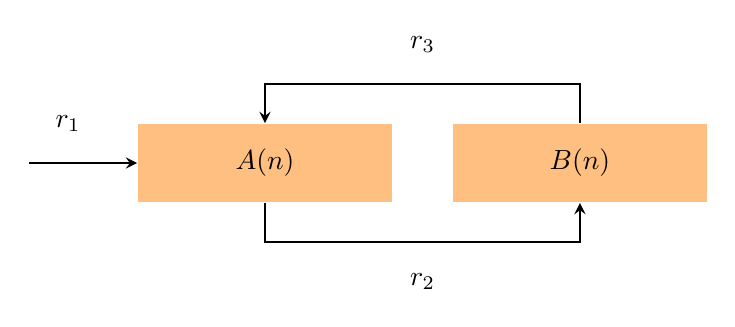
\begin{tikzpicture}
        \node [io] at (2,0) (b) {$B(n)$};
        \node [io] at (-2,0) (a) {$A(n)$};
        \draw [arrow] (a) -- (-2,-1) -- (2,-1) -- (b);
        \draw [arrow] (b) -- (2,1) -- (-2,1) -- (a);
        \draw [arrow] (-5,0) -- (a);
        \node at (-4.5,0.5) {$r_1$};
        \node at (0,-1.5) {$r_2$};
        \node at (0,1.5) {$r_3$};
        \end{tikzpicture}
\end{center}
\begin{center}
    Figure 2: An example of an two-compartment system.
\end{center}

\subsection{Disease Models}

For the following examples, we label the members of a population hit
with an infectious disease as:
\begin{itemize}
	\item Susceptibles ($S$) - members that may become infected.
	\item Infected ($I$) - members that have aquired the disease.
	\item Removed/Recovered ($R$) - members that have recovered
		from the illness, developed an immunity, or possibly
		died (depending on the disease modeled).
\end{itemize}

The model below is known as an SIR model and can be used to model
diseases for which one builds immunity, like chicken pox. The rate
of change from $S$ to $I$ depends on susceptibles coming into
contact with the infected, which is why the rate of change is
proportional to the produce $SI$. The rate of change from $I$ to
$R$ depends on how long the disease lasts, which is why the rate 
is proportional to just $I$.

\begin{center}
    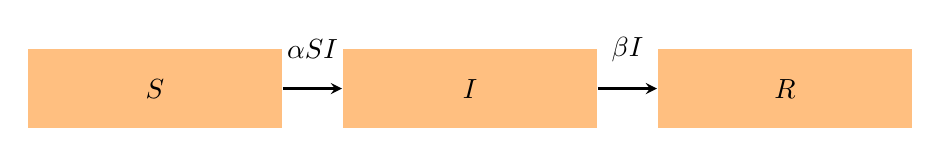
\begin{tikzpicture}
        \node [io] at (0,0) (b) {$I$};
        \node [io] at (-4,0) (a) {$S$};
        \node [io] at (4,0) (c) {$R$};
        \draw [arrow] (a) -- (b);
        \draw [arrow] (b) -- (c);
        \node at (-2,0.5) {$\alpha SI$};
        \node at (2,0.5) {$\beta I$};
        \end{tikzpicture}
\end{center}
\begin{center}
    Figure 3: An SIR model with rates of change.
\end{center}

The next model is an example of an SIR model in which the recovered
population may become susceptible over time, like the flu.

\begin{center}
    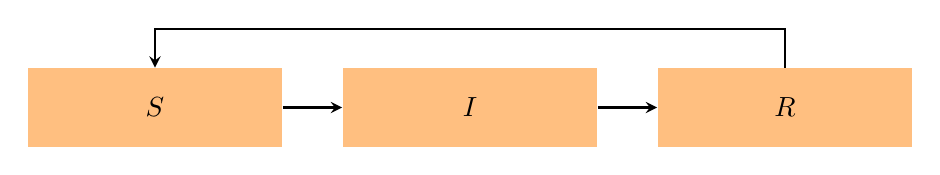
\begin{tikzpicture}
        \node [io] at (0,0) (b) {$I$};
        \node [io] at (-4,0) (a) {$S$};
        \node [io] at (4,0) (c) {$R$};
        \draw [arrow] (a) -- (b);
        \draw [arrow] (b) -- (c);
        \draw [arrow] (c) -- (4,1) -- (-4,1) -- (a);
        \end{tikzpicture}
\end{center}
\begin{center}
    Figure 4: An example of an SIR model with a loss of immunity.
\end{center}

The following model is an example of an SIS model where a population
receives no immunity, like the common cold.

\begin{center}
    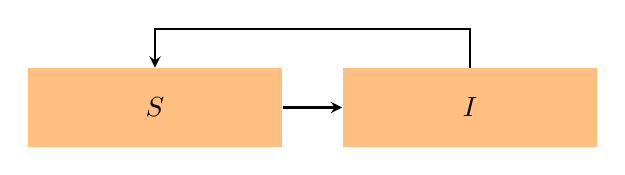
\begin{tikzpicture}
        \node [io] at (2,0) (b) {$I$};
        \node [io] at (-2,0) (a) {$S$};
        \draw [arrow] (a) -- (b);
        \draw [arrow] (b) -- (2,1) -- (-2,1) -- (a);
        \end{tikzpicture}
\end{center}
\begin{center}
    Figure 5: An example of an SIS model.
\end{center}

There is a great paper on modeling the zombie apocalypse with an
interesting model that can be found \href{https://loe.org/images/content/091023/Zombie\%20Publication.pdf}{here}.

\section{Problems}

\begin{question}
A population of 100,000 members is subject to a disease non-fatal disease that leaves individuals immune to future infections. Infection can only occur when a susceptible person comes in direct contact with an infectious person. The infectious period lasts approximately two weeks. It is estimated that 15\% of the population is currently immune to the disease due to a previous exposure. There were 20 reported cases of the disease last week and this week there are 50 new cases of the disease. Plot the number of susceptibles, infected, and recovered individuals over time. Note that in this case,
the hint contains the solution.
\begin{hint}
	\begin{sageCell}
	# SIR model problem solution

	\end{sageCell}
\end{hint}
\end{question}

\end{document}
